
\hypertarget{working_rterm}{}
\section{Rterm interface}
\index{Rterm!interface}

\begin{figure}[H]
  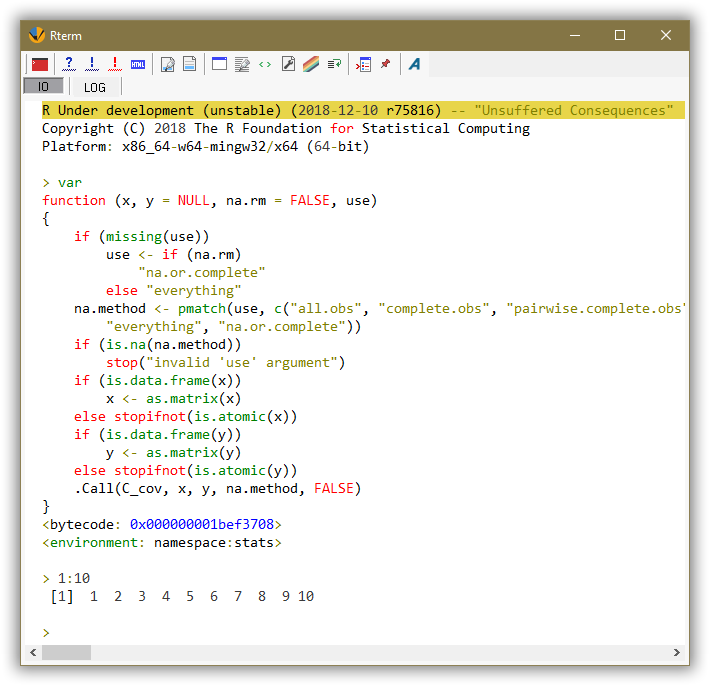
\includegraphics[scale=0.35]{./res/rterm.png}\\
  \caption{Rterm interface.}
  \label{fig:rterm_interface}
\end{figure}

The implementation of a Rterm interface
(Figure \ref{fig:rterm_interface},
\ref{fig:rterm_io} and
\ref{fig:rterm_log})
in Tinn-R has the following aims:
\begin{itemize}
  \item To address some limitations (edition, navigation and control) imposed by the Rgui.exe interface;
  \item To add more flexibility and power to the GUI/Editor;
  \item To maintain the prior user knowledge associated with Tinn-R editor and the Rgui console;
  \item To maintain the structural simplicity of the application;
  \item To use a more efficient engine of Inter Process Communication (IPC)
    than the Windows clipboard used in previous versions.
\end{itemize}

The \textit{IO}
(Figure \ref{fig:rterm_io})
and \textit{LOG}
(Figure \ref{fig:rterm_log})
interfaces are instances of the class
SynEdit. In other words, all prior user knowledge of the resources associated with the editor were preserved:
\index{SynEdit}

\begin{itemize}
  \item Free navigation with keyboard keys;
  \item Marks;
  \item Shortcuts;
  \item Syntax;
  \item Match brackets;
  \item Tips;
  \item Data completion;
  \item Edition: copy, paste, cut, etc;
  \item Selection/copy/paste in column mode:
    \texttt{ALT + drag the mouse}, if this option is checked
    (\htmladdnormallink{see editor options}{\#working\_editor}), etc.
\end{itemize}

\begin{enumerate}
  \item \textit{IO} (Figure \ref{fig:rterm_io}): The aim was to add flexibility and power, i.e.,
    joining the power of SynEdit (editor) and the functionality of
    a common console.
  \item \textit{LOG} (Figure \ref{fig:rterm_log}): Has three basic objectives:
    \begin{enumerate}
      \item To receive and show warnings and error messages;
      \item To make the \textit{IO} interface cleaner;
      \item To avoid synchronization difficulties with the inter
        process communication (IPC) called \textit{pipe} used.
    \end{enumerate}
\end{enumerate}

When more than one recognized instance of \RR{} is running the priority
order is:

\begin{enumerate}
  \item Rterm;
  \item Rgui;
  \item Rserver (remote);
\end{enumerate}


\hypertarget{working_rterm_io}{}
\subsection{IO}
\index{Rterm!IO}
\index{IO Interface}

\begin{figure}[H]
  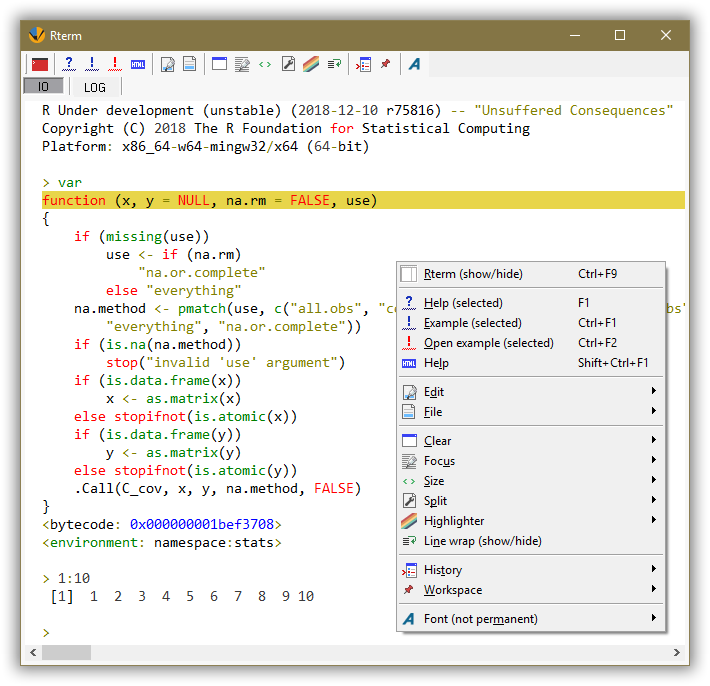
\includegraphics[scale=0.35]{./res/rterm_io.png}\\
  \caption{IO (Rterm interface).}
  \label{fig:rterm_io}
\end{figure}

\begin{table}
  \begin{footnotesize}
    \begin{tabularx}{\textwidth}{>{\hsize=0.3\hsize}X>{\hsize=0.7\hsize}X}\\
      \hline
      \textbf{Resource} & \textbf{Description} \\
      \hline
      Edition & All resources available to the editor (copy, paste, cut, etc) can be used \\
      Free navigation & Using keyboard keys: Home, Page Up, Page Down, End, Left, Top, Right and Bottom \\
      Marks & \texttt{CTRL + [0..9]} can be used to mark, \texttt{SHIFT + CTRL + [0..9]} to go to prior marks \\
      Shortcuts & All shortcuts available to the editor are also to the IO \\
      Syntax & Two options: Text and \RR{} \\
      Match brackets & Makes it easier to build more complex instructions like \texttt{plot(sqrt(rnorm(1e3)), pch='.', cex=3)} \\
      Tips & Are invoked using the same trigger as the editor \\
      Data completion & Are invoked using the same trigger as the editor \\
      \hline
      \\
    \end{tabularx}
  \end{footnotesize}
  \caption{IO interface, main resources available.}
  \label{tab:io_interface}
\end{table}

The \textit{IO} interface
(Figure \ref{fig:rterm_io} and
Table \ref{tab:io_interface})
is used to receive output (SDTOUT) from the \RR{} environment.

It is necessary to adjust some \RR{} options (for example: \texttt{options(width=70)}
to obtain a suitable number of characters in each single line, according to
hardware and user preferences (side of \textit{IO}, place of \textit{IO},
length of \textit{IO}, width of \textit{IO}, type and size of font). Once
you get a suitable result, it is a good practice to add this option to the
\texttt{Rprofile.site} (located inside of the folder \textit{etc} where the
\RR{} was installed) file. Thus, your option will always be set when
starting \RR{}.

The IO is an instance of SynEdit. Therefore, it can be edited and used like
the editor, allowing the tasks showed in the
Table \ref{tab:io_interface}.

If the \textit{IO} has the focus, all actions of the \RR{} toolbar and main menu
associated with control \RR{} can be used in the IO interface.

The \textit{IO} interface has a special pop-up menu allowing the most common
tasks. It is self-explanatory. So, make a small tour (right mouse button inside
of Rterm/IO) to find out about its options.

Some details:

\begin{itemize}
  \item Shortcuts and pop-up menu make it easy to change among the interfaces:
    \textit{Editor}, \textit{IO} and \textit{LOG}:
    \begin{enumerate}
      \item if \textit{IO} and \textit{LOG} are in distinct tabs (views), the
        common Windows shortcut \texttt{CTRL + TAB} changes the active page (IO-LOG).
      \item Any prior line can be sent another time by just putting the cursor
        in any place of it and typing: \texttt{CTRL + ENTER};
    \end{enumerate}
  \item The last line of the \textit{IO} interface (the prompt) has special features:
    \begin{enumerate}
      \item \texttt{CTRL+ENTER} must be used to send any line or selection (single line only) to R interpreter;
      \item \texttt{ALT+DOWN} and \texttt{ALT+UP} are the shortcuts (prior/later)
        for command R history. The R history is continuous, cyclic, and have a 100
        line limit.
    \end{enumerate}
\end{itemize}


\hypertarget{working_rterm_log}{}
\subsection{LOG}
\index{Rterm!LOG}
\index{LOG Interface}

 \begin{figure}[H]
  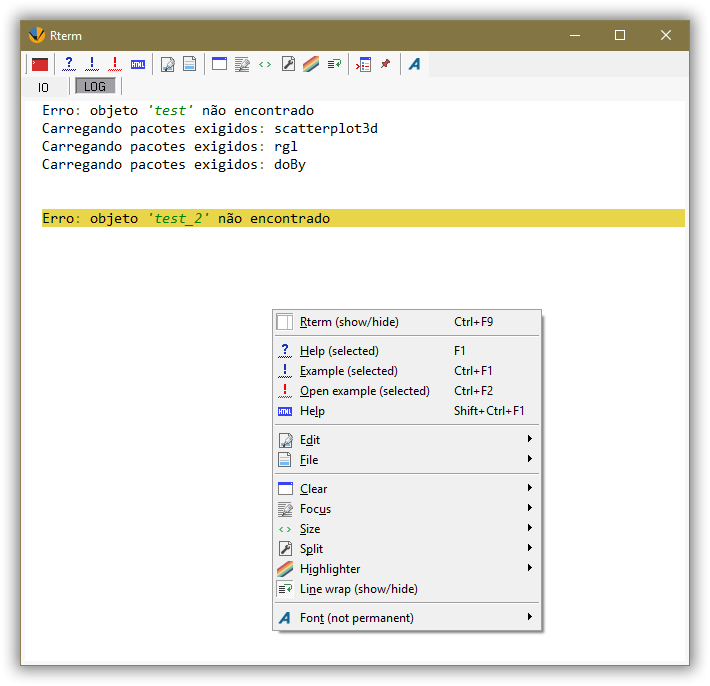
\includegraphics[scale=0.35]{./res/rterm_log.png}\\
  \caption{LOG (Rterm interface).}
  \label{fig:rterm_log}
\end{figure}

The \textit{LOG} interface
(Figure \ref{fig:rterm_log})
is used to receive warnings and error messages (SDTERR) from the \RR{} environment.

It has a special pop-up menu that allows the most common tasks. It is
self-explanatory. So, take a small tour (right mouse buttom inside of
Rterm/LOG) to know all options.

Most of the resources available to the \textit{IO} are also available to this
interface.
